\documentclass[10pt,twocolumn]{article}

\usepackage{lmodern}
\usepackage[T1]{fontenc}
\usepackage[a4paper, top=2.0cm, bottom=2.4cm, left=1.5cm, right=1.5cm, columnsep=0.65cm]{geometry}
\usepackage{amsmath}
\usepackage{booktabs}
\usepackage{graphicx}
\usepackage{microtype}
\usepackage{titlesec}
\usepackage{caption}
\usepackage{xcolor}
\usepackage{url}
\usepackage{fancyhdr}
\usepackage{hyperref}

\graphicspath{{../../figures/}}

\hypersetup{
  colorlinks=true,
  linkcolor=blue!60!black,
  citecolor=blue!60!black,
  urlcolor=blue!60!black,
  pdftitle={Tracing Model-Generated DNA with Position-Independent SynthID Watermarking},
  pdfauthor={Kimon Antonios Provatas; Christos Galanopoulos; Aris Karatzikos; Charalambos Koilakos; Ilias Georgakopoulos-Soares},
  pdfsubject={Position-independent detection of the SynthID tournament watermark in two genomic language models},
  pdfkeywords={genomic language models; watermarking; SynthID; provenance; position-independent detection}
}
\pdfstringdefDisableCommands{\def\texttt#1{#1}}

\titleformat{\section}{\normalfont\large\bfseries}{\thesection}{1em}{}
\titleformat{\subsection}{\normalfont\normalsize\bfseries}{\thesubsection}{1em}{}

\captionsetup{font=small, labelfont=bf}
\raggedbottom
\setlength{\emergencystretch}{2em}

%% full-width floats in two columns can only float forward to a page top;
%% loosen the defaults so they land near their reference instead of drifting
\setcounter{topnumber}{2}
\setcounter{dbltopnumber}{2}
\renewcommand{\dbltopfraction}{0.9}
\renewcommand{\dblfloatpagefraction}{0.7}
\renewcommand{\textfraction}{0.07}

\pagestyle{fancy}
\fancyhf{}
\fancyfoot[R]{\small\thepage}
\renewcommand{\headrulewidth}{0pt}
\renewcommand{\footrulewidth}{0.4pt}

\begin{document}

\twocolumn[{%
\begin{center}
{\LARGE\bfseries Tracing Model-Generated DNA\\[3pt]
with Position-Independent SynthID Watermarking\par}
\vspace{1.0em}
{\large
Kimon Antonios Provatas\textsuperscript{1,*}\hspace{0.9em}
Christos Galanopoulos\textsuperscript{1,*}\hspace{0.9em}
Aris Karatzikos\textsuperscript{1}\\[4pt]
Charalambos Koilakos\textsuperscript{1}\hspace{0.9em}
Ilias Georgakopoulos-Soares\textsuperscript{1,\dag}\par}
\vspace{0.6em}
{\footnotesize
\textsuperscript{1}The University of Texas at Austin, Austin, Texas, USA\\[2pt]
\textsuperscript{*}These authors contributed equally.\quad
\textsuperscript{\dag}Correspondence: \href{mailto:ilias@austin.utexas.edu}{ilias@austin.utexas.edu}\par}
\vspace{1.4em}
\begin{minipage}{0.86\textwidth}
\small
\textbf{Abstract.}
Genomic language models can generate DNA sequences that resemble naturally occurring genomic
material, yet the resulting sequences contain no inherent record of their origin. A watermark
embedded during sequence generation can enable a holder of the corresponding secret key to
identify model-generated output subsequently. In DNA, however, unknown generation boundaries,
token alignment, and strand orientation complicate detection, particularly when generated sequence
is embedded within a longer read.

We integrate the SynthID tournament watermark into Carbon-500M and GENERator-v2 1.2B, two genomic
language models that generate non-overlapping six-base tokens, and evaluate sampler fidelity,
sequence-quality proxies, and position-independent detection. Neither model exhibited a
statistically detectable difference in model likelihood or the pre-specified sequence measures
after multiple-testing correction. The verifier requires the DNA, the key, and fixed public
settings, and controls the read-level test through a correction over both strands, every starting
base, and four window lengths. In each model, it detected all 384 held-out marked reads in the
unedited condition and after each tested single-base substitution, insertion, or deletion. Ordinary
and wrong-key controls yielded at most one positive per model, control family, and condition. Carbon
window-level analyses support recovery of token alignment through the search after an insertion or
deletion. These findings support the portability of the implementation across the two evaluated
models. They establish statistical detection within the tested corpus, without establishing
biological function or resistance to secret-key recovery. Each model was evaluated in a single
execution; independent confirmatory replication remains outstanding.
\end{minipage}
\vspace{1.2em}
\end{center}
}]

\thispagestyle{fancy}

\section{Introduction}

Genomic language models increasingly support the generation of coding sequences, regulatory
elements, and extended genomic sequences \cite{nguyen2024evo,wu2025generator,carbon2026}. As these
capabilities develop, establishing the provenance of generated DNA becomes an important component
of responsible sequence design and synthesis. A nucleotide sequence alone does not inherently
specify whether it originated from a biological sample, a computational design process, or a
generative model. Once a sequence is separated from its associated metadata, records maintained by
the generating software may no longer be available to downstream users. Provenance mechanisms that
remain associated with a sequence throughout design and synthesis have consequently attracted
attention \cite{baker2024protein}.

Watermarking provides one approach to this problem by embedding a statistical signal during
generation. A verifier with the corresponding secret key can subsequently test for that signal
without access to the generating model, the prompt, or generation logs. Adapting language-model
watermarking to DNA introduces a specific alignment problem. For a model that generates
non-overlapping six-base tokens, the nucleotide sequence does not explicitly encode the token
boundaries. An unknown generation boundary therefore introduces six possible token alignments.
Reverse complementation adds uncertainty in strand orientation, and embedding generated sequence
within a longer read introduces uncertainty in its location and extent. Detection must account for
all searched alternatives when controlling the read-level false-positive rate; a significant
result at a known alignment need not remain significant after this correction.

Here, we integrate the SynthID tournament watermark \cite{dathathri2024scalable} into Carbon-500M
\cite{carbon2026} and GENERator-v2 1.2B \cite{generatorv22026}. These models share six-base
tokenisation but differ in size, training corpus, and tokenizer construction. We evaluate two
questions: whether watermarking produces detectable changes in each model's likelihood and a
pre-specified panel of sequence statistics, and whether a verifier can detect the mark without
knowing the generation boundary, strand orientation, or token alignment. The verifier searches
both strands, every starting base, and multiple window lengths, with a single read-level
multiple-testing correction covering the complete search.

Neither model exhibited a statistically detectable change in the evaluated quality proxies. The
verifier detected every held-out marked read in both models, including after each tested
single-base substitution, insertion, or deletion. Ordinary and wrong-key control counts were
compatible with the declared false-positive target, although their confidence intervals do not
establish an operational rate below that target. In Carbon, retained window-level results further
show substantial separation from the corrected threshold and a shift toward shorter detection
windows after insertions and deletions. These findings support application of the same sampler and
verifier to two genomic models; they do not establish equivalence between the models or their
generated sequences.

The analysis distinguishes mathematical identities of the watermark construction, cryptographic
modelling assumptions, empirical detection results, and sequence-based quality proxies. In
particular, preservation of the model distribution is an expectation over fresh keyed functions;
sampling at a fixed key and context follows a deliberately reweighted distribution. Model
likelihood and sequence statistics do not establish biological function, viability, or safety, and
the experiments do not evaluate resistance to secret-key recovery. Table~\ref{tab:vocabulary}
defines the terminology and notation used throughout the paper.

\begin{table*}[t]
\centering
\caption{Terminology and notation used throughout the paper.}
\label{tab:vocabulary}
\small
\begin{tabular}{ll}
\toprule
Word or symbol & Meaning \\
\midrule
model             & either of the two used here, each restricted to its 4{,}096 six-base DNA tokens \\
Carbon            & Carbon-500M \\
GENERator         & GENERator-v2-eukaryote-1.2b-base \\
token             & a non-overlapping DNA sequence of six bases \\
prompt            & a 384-base RefSeq sequence supplied to the model \\
continuation      & the 3{,}072 bases generated by the model \\
read              & what the verifier receives: prompt and continuation, $N = 3{,}456$ bases \\
mark              & the SynthID tournament watermark \\
key, $k$          & the secret used for watermark embedding and detection \\
published key     & a key released with this study so the runs can be reproduced \\
mark bit, $g$     & a keyed value of 0 or 1 for one candidate token in one context \\
layer, $m$        & one keyed round of the tournament; $m = 30$ layers are applied \\
context           & the four tokens generated immediately before the current one \\
$p$               & the model's probability for a candidate token \\
$p_k$             & the probability the sampler actually uses, after the $m$ layers \\
window            & a contiguous region of the read scored by the verifier \\
$L$               & window length in bases; $L \in \{384,\, 768,\, 1{,}536,\, 3{,}072\}$ \\
$M$               & windows searched in one read; $M = 16{,}136$ for $N = 3{,}456$ \\
$n$               & mark bits scored inside a window \\
$S$               & the number of scored bits equal to 1 \\
$P_{\mathrm{win}}$  & the binomial-tail probability for one window \\
$P_{\mathrm{read}}$ & the read-level $P$-value after correction over all searched windows \\
window strength   & $-\log_{10} P_{\mathrm{win}}$, so larger means stronger evidence \\
recall            & proportion of marked reads with a positive detection \\
false-positive rate & proportion of control reads with a positive detection \\
$\alpha$          & the target false-positive rate for one read; $\alpha = 0.01$ \\
ordinary          & sampled directly from $p$, without a key \\
draw              & one of the two continuations generated per prompt in each model \\
\bottomrule
\end{tabular}
\end{table*}

\section{Background}

\subsection{Watermarking designed DNA}

DNA watermarking predates its application to generative models. The first synthetic bacterial
genome included watermark sequences encoding identifying information to distinguish the synthetic
chromosome from its natural counterpart \cite{gibson2010creation}. DNA-Crypt formalised message
embedding through synonymous codon choices and error correction \cite{heider2007dna}. Related
approaches embed information within an open reading frame while preserving the encoded amino acid
sequence, with experimental evidence that embedded messages can persist during viral replication
\cite{liss2012watermarks}.

These approaches rely on explicit sequence design, through either insertion of a payload or
modification of selected nucleotides. Their application requires suitable locations for embedding
and consideration of the biological consequences of those changes. Generation-time watermarking
addresses a complementary setting: the mark is introduced through the model's sampling
distribution as the sequence is generated, without requiring a separately allocated payload
region. A fixed, recognisable marker also differs from a distributed keyed signal in its
susceptibility to targeted removal or copying.

\subsection{Watermarking language-model output}

Language-model watermarking modifies token sampling to introduce a statistically detectable
pattern. A widely studied approach partitions the vocabulary into pseudorandom green and red
lists, increases the probability of green-list tokens, and detects the mark through their excess
frequency \cite{kirchenbauer2023watermark}. This modification changes the sampling distribution
and can introduce a tradeoff between detection strength and generation quality.

Other constructions preserve the model distribution in expectation over fresh keyed randomness.
Cryptographic formulations establish computational indistinguishability from ordinary output
under specified assumptions \cite{christ2024undetectable}. Practical approaches use
inverse-transform or exponential-minimum sampling and align the observed output against a keyed
random sequence during detection \cite{kuditipudi2024robust,aaronson2022watermark}. Another family
directly reweights the token distribution while recovering the original distribution in
expectation \cite{hu2024unbiased,wu2024dipmark}; SynthID uses this general principle. Publicly
verifiable constructions instead embed a signature through rejection sampling, subject to
sufficient output entropy \cite{fairoze2025publicly}.

Robustness depends on the assumed adversary and permitted edits. Theoretical results identify
limitations under sufficiently capable quality-preserving rewriting attacks \cite{zhang2024sand}.
Empirical studies demonstrate evasion through adaptive or recursive paraphrasing
\cite{diaa2025adaptive,sadasivan2025reliably}, watermark forgery and removal through model queries
\cite{jovanovic2024stealing}, and recovery of keyed sequences through adaptive prompting
\cite{reynolds2025breaking}. Reuse of keyed randomness can also compromise distributional
preservation \cite{wu2024collisions}. Countermeasures for detecting spoofed watermarks have been
investigated \cite{gloaguen2025spoofing}. The present study evaluates statistical detection under
single-base edits and does not test these adversarial capabilities.

\subsection{SynthID}

We use the binary tournament construction of SynthID-Text \cite{dathathri2024scalable}. At each
generation step, a secret key and a short context of recently generated tokens determine binary
mark bits for each candidate token and tournament layer. Each layer favours candidates with a
mark bit of 1. Averaged over fresh keyed functions, the tournament preserves the model's
next-token distribution; at a fixed key and context, it samples from a reweighted distribution.
Detection reconstructs the mark bits from the output and tests for an excess of 1s.

Two properties motivate this construction for genomic sequences. First, the mark bits depend on
local token context rather than absolute position, allowing detection to use contexts retained
when a generated region is relocated or cropped. Second, the detector requires the output, key,
and public settings without access to the generating model or its probabilities. SynthID-Text has
also been evaluated in a large-scale text deployment \cite{dathathri2024scalable}.

\subsection{Genomic tokenisation and alignment}

Genomic language models support both representation learning and sequence generation
\cite{dallatorre2025nucleotide,nguyen2024evo}. Several generative models, including both evaluated
here, tokenise DNA into non-overlapping six-base tokens to reduce token-sequence length
\cite{wu2025generator,carbon2026,generatorv22026}. Some models additionally obtain single-base
probabilities by marginalising the token distribution \cite{generatorv22026}. The released
GENERator checkpoint includes a base-by-base sampling path \cite{generatorv2checkpoint}; the
present study instead uses its direct canonical six-base token distribution, as specified below.

Six-base tokenisation introduces alignment uncertainty because token boundaries are not explicitly
represented in the nucleotide sequence. A verifier must therefore consider all six possible
alignments, both strand orientations, and the possible locations and lengths of a generated
region. Selecting the strongest window without correcting for this search would overstate the
statistical evidence. We consequently evaluate detection using a read-level correction over the
complete search.

Recent work on genomic watermarking uses synonymous codon substitution to mark designed coding
sequences and propagate the mark into translated proteins \cite{zhang2025securing}. Related work
applies keyed reweighting to protein generation to support local verification of authorised
provenance \cite{chen2025protein}. Our setting addresses detection in DNA without assuming that
the generated region is coding, that a reference alignment is available, or that its boundary is
known. We evaluate an established watermark construction under these conditions using only the
observed read, a key, and public detector settings.

\section{Methods}

\subsection{Model and sampling}

Generation used Carbon-500M
\cite{carbon2026,carbon500m} and GENERator-v2-eukaryote-1.2b-base
\cite{generatorv22026,generatorv2checkpoint}. Both are decoder-only genomic language models that
tokenise DNA into non-overlapping six-base tokens and differ in size, training corpus, and
tokenizer construction. Both models were evaluated separately under the same core generation,
sampler-validation, sequence-quality, and detection procedures. Results are reported per model.

At each step the model's logits were restricted to the 4{,}096 canonical DNA tokens and normalised
once, which for GENERator means its direct canonical token distribution rather than the base-by-base
path its released code uses by default. Temperature was 1.0 and no top-$k$ or top-$p$ truncation was
applied. The ordinary arm samples from that distribution directly and uses no key. The marked arm
applies the tournament described below and then samples.

Generation ran on GPU hardware. Model scoring ran on CPU for Carbon and on GPU for GENERator, and
detection ran on x86-64 CPUs for both.

\subsection{Watermark embedding}

At each generation step, the model assigns probability $p$ to each of 4{,}096 tokens. The key,
the preceding four tokens of context, and the candidate token determine its binary mark bit $g$.
Mark bits are derived with HMAC-SHA-256 over the key, a fixed domain label, the context, and the
candidate token. The tournament formula, the number of layers, the context width, and the
repeated-context rule follow the public reference implementation of
SynthID-Text \cite{synthidtextcode}. One tournament layer reweights the distribution as
\begin{equation}
p'(x) \;=\; p(x)\,\Bigl(1 + g(x) - \textstyle\sum_y p(y)\, g(y)\Bigr),
\label{eq:layer}
\end{equation}
so that candidates with a mark bit of 1 gain probability according to the total probability mass
assigned to such candidates. Iterating this update is equivalent to evaluating the binary
tournament without explicitly constructing its $2^{m}$ leaves. The sampler applies $m = 30$
layers, each with its own mark bits, and samples a token from the resulting distribution $p_k$
(Figure~\ref{fig:method}a).

The first four generated tokens are sampled ordinarily so that subsequent watermark contexts can
be reconstructed from the continuation alone. A repeated four-token context is also sampled
ordinarily and excluded from the detector score, following the original construction. A history
of 1{,}024 contexts is maintained for repetition detection.

Averaged over fresh keyed functions, Equation~\ref{eq:layer} leaves the model's next-token
distribution unchanged. This identity does not imply equality at a fixed key and context, where
the sampler follows the explicitly reweighted distribution $p_k$. Sampler fidelity was therefore
evaluated against $p_k$.

\subsection{Position-independent detection}

The verifier receives the read, the key, the generation domain label, and fixed public detector
settings. It does not receive the prompt, the model, the model's probabilities,
the seed, the strand orientation, the token alignment, or the generation boundary
(Figure~\ref{fig:method}b).

For each of the four window lengths $L$ that fit within the read, the verifier evaluates every
starting base on the supplied strand and its reverse complement. This search covers candidate
generation boundaries and all six token alignments. Within each window, DNA is partitioned into
tokens relative to the window start. The first four tokens provide context; the verifier
reconstructs mark bits for the remaining eligible tokens and obtains $S$ ones among $n$ scored bits.

Under the null assumption that mark bits behave as independent fair binary values, the
window-level $P$-value is the exact binomial tail
\begin{equation}
P_{\mathrm{win}} \;=\; \Pr\bigl[\mathrm{Binomial}(n, \tfrac{1}{2}) \geq S\bigr].
\end{equation}
The verifier scores $M = 2\sum_L (N - L + 1)$ windows, which is 16{,}136 for a 3{,}456-base read,
and reports a single read-level result:
\begin{equation}
\begin{aligned}
P_{\mathrm{read}} &\;=\; \min\bigl(1,\; M \cdot \min_{\text{windows}} P_{\mathrm{win}}\bigr),\\
\text{mark found} &\iff P_{\mathrm{read}} \leq \alpha .
\end{aligned}
\end{equation}
The Bonferroni correction by $M$ accounts for all searched windows, including overlapping windows,
without requiring independence between their tests. The threshold uses the pre-specified
$\alpha = 0.01$ and is not fitted to the evaluated reads. Equivalently, a read is positive only if
at least one window reaches
strength $\log_{10}(M/\alpha) = 6.21$. Window lengths are 384, 768, 1{,}536 and 3{,}072 bases; a
window whose length does not fit the read is not searched, and a read shorter than every
pre-specified
length is not scored. Reverse-complement coordinates are mapped back onto the supplied read, and
log-probabilities are retained throughout to avoid floating-point underflow.

\begin{figure*}[t]
\centering
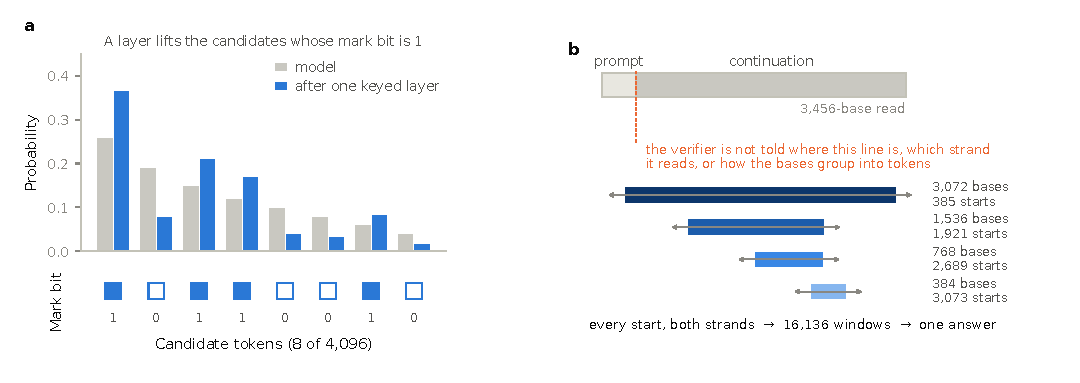
\includegraphics[width=\textwidth]{fig1_method}
\caption{\textbf{SynthID embedding and position-independent detection.}
\textbf{a}, One keyed layer, drawn for eight of the 4{,}096 candidate tokens with an illustrative
distribution. Candidates whose mark bit is 1 gain probability; the others lose it. The sampler
applies 30 such layers.
\textbf{b}, Detector inputs and search. The verifier receives the read, key, and fixed public
settings without the generation boundary, strand orientation, or token alignment. It scores
windows of four lengths at every starting base on both strands, comprising 16{,}136 windows for a
3{,}456-base read, and reports one read-level result corrected for the full search. Panel
\textbf{a} illustrates
Equation~\ref{eq:layer} and is not a measurement.}
\label{fig:method}
\end{figure*}

\subsection{Prompts and generation}

Both models use the same cohort of 256 prompts: 384-base forward-strand windows drawn
from 16 accession-versioned RefSeq chromosome records across eight model organisms. Windows were
chosen by hashing a fixed label, the
accession, and a segment index, before generation. Human, patient, controlled-access,
organelle, plasmid, and ambiguous-base spans were excluded. No prompt was added, moved, or removed
after any model was run.

In each model, each prompt produced two marked and two ordinary continuations of 512 tokens
(3{,}072 bases), so each model contributes 512 marked and 512 ordinary continuations. The
two draws use different replay seeds in both arms, and the two marked draws use two different keys.
Both keys are published for reproducibility. Deployment would require independently generated
secret keys shared only with authorised generators and verifiers.

\subsection{Sampler validation}

For each model and prompt we fixed the model at token index 64 of its ordinary draw-zero trajectory
and drew 5{,}000 samples per arm from that one state. Counts were compared with the exact intended
law by a
Monte Carlo goodness-of-fit test with 999 replicates. The marked arm was compared against $p_k$, not
against $p$, because the distribution-preservation identity does not hold at a fixed key and
context. Eight additional states per model used a deliberately incorrect sampler as a negative
control.

\subsection{Sequence measures}

The model's score is the teacher-forced negative log-likelihood per generated token under the same
model and token restriction used to generate, with the prompt supplied as context and excluded from
the loss. Each model scores its own outputs, so the absolute scores are not used for comparisons
between models. Thirteen additional measures were specified before analysis: GC content,
purine content, CpG
content, base, dinucleotide and trinucleotide entropy, distinct 6-mer fraction, longest and mean
single-base run, Jensen--Shannon drift from the prompt at $k = 1, 2, 3$, and perplexity. All 14 form
one multiple-testing family under Benjamini--Hochberg correction.

\subsection{Edits and statistics}

Each edited read contains exactly one substituted, inserted, or deleted base within the continuation,
at a position and with a replacement base drawn by a fixed random rule that does not consult the
verifier. Prompts are the independent unit; the two draws from a prompt are paired repetitions.
Uncertainty on the sequence measures comes from an equal-weight bootstrap over prompts with 20{,}000
replicates and a paired sign-flip test with 100{,}000 replicates. Detection intervals are exact
two-sided binomial intervals at 95\% over the 192 held-out prompts. For control families, a prompt
is positive if either draw is positive; marked-output recall is also assessed by requiring both
draws to be detected. All reported read-level $P$-values include the correction over every searched
strand, starting base, and window length.

\section{Results}

\subsection{Sampler fidelity}

We first evaluated agreement between each sampler and its intended distribution. Of 256
marked states, 13 fell below the nominal 0.05 level in Carbon and 5 in GENERator, against 12.8
expected by chance in each model; the ordinary arms gave 12 and 14. No arm in either model produced
a rejection after correction, while all eight states evaluated with a deliberately incorrect
sampler were rejected in each model. These results support sampler fidelity at the 256 evaluated
states and the resolution provided by 5{,}000 draws per state. They do not constitute a proof of
correctness at all possible model states.

\subsection{Sequence-quality proxies}

For every prompt and model we generated two marked and two ordinary continuations of 3{,}072 bases
under the same conditions, giving 512 matched pairs from 256 prompts in each model.

In Carbon the model's own score was 7.53386 nats per token for ordinary output and 7.54238 for
marked output. The paired difference is $+0.00852$ nats per token, with a 95\% interval from
$-0.04426$ to $+0.05973$ and $P = 0.75$ (Figure~\ref{fig:quality}a); as a standardized effect that
is 0.0201. In GENERator the score was 7.80029 for ordinary output and 7.79465 for marked output, a
paired difference of $-0.00564$ nats per token, with a 95\% interval from $-0.05614$ to $+0.04378$,
$P = 0.83$, and a standardized effect of $-0.0139$. The paired differences have opposite signs,
and neither confidence interval excludes zero.

The thirteen further measures, covering base composition, $k$-mer entropy, distinct 6-mers,
single-base runs, CpG content, and compositional drift from the prompt, also show no statistically
detectable differences in either model. All 14 intervals contain zero, no comparison is significant
after multiple-testing correction, and the smallest adjusted $P$-value is 0.85 in Carbon and 0.73
in GENERator. For Carbon the
largest effect in absolute value is 0.084 standard deviations (Figure~\ref{fig:quality}b); the
equivalent summary was not retained for GENERator, for which the supported conclusion is the
absence of significant differences after correction.

These results indicate no measurable quality loss under the evaluated proxies. They do not
establish equivalence: the model-score confidence intervals permit changes on the order of
0.05 nats per token. Moreover, model likelihood and sequence statistics do not measure biological
function, and absolute likelihood scores are not directly comparable between the two models.

\begin{figure*}[t]
\centering
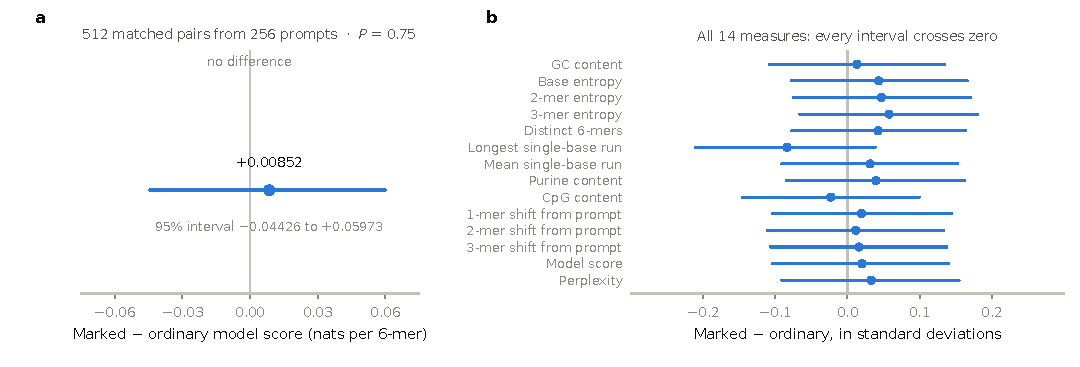
\includegraphics[width=\textwidth]{fig2_quality}
\caption{\textbf{Model likelihood and sequence-quality proxies for Carbon.} All panels are Carbon; the
GENERator summaries are reported in the text only.
\textbf{a}, Paired difference in the model's score between marked and ordinary continuations, over
512 matched pairs from 256 prompts. Positive values indicate lower model likelihood for marked
continuations. The bar denotes the 95\% interval from a bootstrap over prompts.
\textbf{b}, All 14 pre-specified measures on one scale, as the paired difference in standard
deviations, with confidence intervals rescaled to the same units. Every interval includes zero,
and none of the 14 comparisons is significant after multiple-testing correction.}
\label{fig:quality}
\end{figure*}

\subsection{Recall and false-positive rate}

The prompt split was specified before examining detection results: 64 prompts were reserved for
selection between two window-score summaries, and 192 were held out for evaluation. Neither subset
was used to fit the threshold. For each model, the 384-base prompt was prepended to each held-out
continuation, producing a 3{,}456-base read whose generation boundary was withheld from the
verifier. Three detection families were evaluated: marked reads with the correct key, ordinary
reads, and marked reads with the other draw's key. Each family was evaluated unedited and after
exactly one substitution, insertion, or deletion. The search depends on read and window lengths
and is identical across models. Unedited reads require $M = 16{,}136$ windows and a threshold of
6.21; the window count is recomputed for the read length after an edit.

In both models, the verifier detected 384 of 384 marked reads in all four conditions
(Table~\ref{tab:detection}), a recall of 100\% per model. The control positives occurred in
different families. In Carbon, one of 384 ordinary reads was positive and no wrong-key read was
positive. In GENERator, no ordinary read was positive and one of 384 wrong-key reads was positive
in the unedited,
substituted, and inserted conditions but not the deleted one. Each of those single positives is a
false-positive rate of 0.26\% in its cell. We report recall and the two false-positive rates
separately because pooled accuracy would depend on the chosen proportions of marked, ordinary,
and wrong-key reads in the evaluation cohort.

Carbon showed substantial separation between marked and control reads. On unedited reads, the
weakest marked read reached window
strength 124.8, while the strongest ordinary read reached 6.60 and the strongest wrong-key read
reached 5.69, against a threshold of 6.21 (Figure~\ref{fig:detection}a). The single ordinary read
that was positive exceeded the threshold slightly. This observation is compatible with occasional
false positives under the declared $\alpha = 0.01$, but does not independently establish
calibration. The window-strength distribution was not retained for GENERator, so threshold margins
and the edit-specific strengths below are reported for Carbon only.

Confidence intervals account for paired draws by using the prompt as the independent unit. In
each model, all 192 prompts had both marked draws detected, giving an exact 95\% interval of
98.10--100\%. In Carbon one
prompt of 192 produced an ordinary positive, giving 0.013--2.868\%, and none produced a wrong-key
positive, giving an upper bound of 1.903\% (Figure~\ref{fig:detection}b). In GENERator, no prompt
produced an ordinary positive, giving an upper bound of
1.903\%, and one produced a wrong-key positive, 0.013--2.868\%. Within each model, control positives
across conditions refer to the same prompt and draw. Carbon's ordinary read remained positive in
all four conditions because each edit occurred outside its strongest window. GENERator's wrong-key
read remained positive after substitution and insertion, but not after deletion.

GENERator also provides a diagnostic assessment of the analytic null under known token alignment.
Scoring ordinary output over the full 256-prompt cohort, the number of
prompts producing a positive was 2, 6, 6 and 4 at the four window lengths, against about five
expected at each, with exact two-sided $P$-values of 0.25, 0.87, 0.76 and 0.84. The analytic null
is therefore compatible with the ordinary-output counts at each evaluated length. This diagnostic
was performed for GENERator only and does not replace the full-search correction.

\begin{table*}[t]
\centering
\caption{Positive detections for each model across 192 held-out prompts with two draws each.
Each edit affects exactly one base. The final two rows of each block summarise unedited reads at
the prompt level, accounting for paired draws; intervals are exact and two-sided. All marked
prompts also had both draws detected in every edit condition. Results are reported separately
for each model.}
\label{tab:detection}
\begin{tabular}{lccc}
\toprule
Edit applied to the read & Marked, right key & Ordinary & Marked, wrong key \\
\midrule
\multicolumn{4}{l}{\emph{Carbon}} \\
None                 & 384/384 & 1/384 & 0/384 \\
One substitution     & 384/384 & 1/384 & 0/384 \\
One insertion        & 384/384 & 1/384 & 0/384 \\
One deletion         & 384/384 & 1/384 & 0/384 \\
Prompts with a positive draw & 192/192 & 1/192 & 0/192 \\
Exact 95\% interval  & 98.10--100\% & 0.013--2.868\% & 0--1.903\% \\
\midrule
\multicolumn{4}{l}{\emph{GENERator}} \\
None                 & 384/384 & 0/384 & 1/384 \\
One substitution     & 384/384 & 0/384 & 1/384 \\
One insertion        & 384/384 & 0/384 & 1/384 \\
One deletion         & 384/384 & 0/384 & 0/384 \\
Prompts with a positive draw & 192/192 & 0/192 & 1/192 \\
Exact 95\% interval  & 98.10--100\% & 0--1.903\% & 0.013--2.868\% \\
\bottomrule
\end{tabular}
\end{table*}

\begin{figure*}[t]
\centering
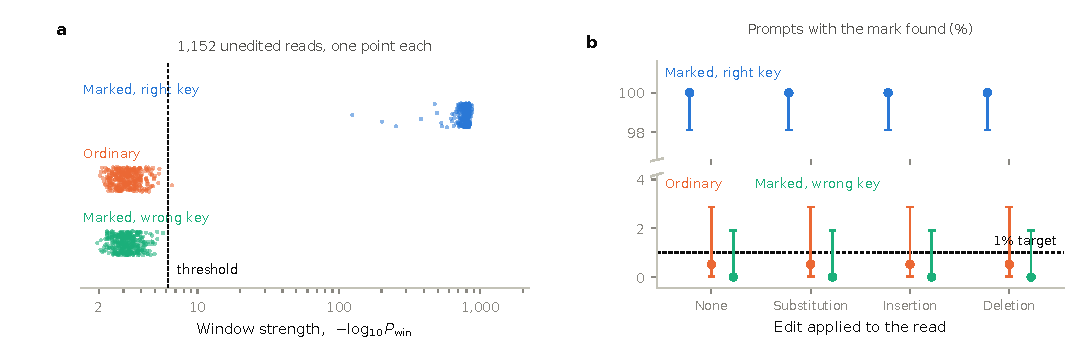
\includegraphics[width=\textwidth]{fig3_detection}
\caption{\textbf{Position-independent detection in Carbon.} All panels
are Carbon; GENERator's decisions are in Table~\ref{tab:detection}, and its window strengths were
not retained.
\textbf{a}, Strength of the best window in each unedited read, one point per read, on a log scale.
The dashed line denotes the threshold corrected for the search over 16{,}136 windows. All marked
reads exceed the threshold; one ordinary read is also positive, whereas all wrong-key reads remain
below it.
\textbf{b}, Proportion of the 192 held-out prompts with positive detections, with exact 95\%
intervals, split across a break in the axis. Results are the same in all four edit conditions. The
control intervals reach above the 1\% target, so these data are consistent with a false-positive
rate below 1\% without establishing one.}
\label{fig:detection}
\end{figure*}

\subsection{Detection after single-base edits}

Window-level analyses are available for Carbon. A substitution perturbs token content and nearby
watermark contexts while preserving downstream token alignment. The median window strength
decreased from 790.6 for unedited reads to 774.7 after substitution
(Figure~\ref{fig:edits}a). Insertions and deletions shift downstream token alignment, reducing the
signal in windows that span the edit.

For unedited reads, the full 3{,}072-base window provided the strongest evidence in 383 of 384
reads. After insertion, that count decreased to 203, with 181 reads favouring a shorter window;
after deletion, the corresponding counts were 232 and 152 (Figure~\ref{fig:edits}b). Searching
every starting base allows windows downstream of the edit to recover the original token alignment.
The observed shift toward shorter windows is consistent with detection using regions whose
alignment is preserved or recovered. Median strength decreased to 431.5 after insertion and 443.7
after deletion. The weakest marked read across all conditions still reached 82.2, above the
threshold of 6.21, and every marked read remained detectable.

GENERator's retained results establish detection outcomes without the corresponding window-level
analysis. All 384 marked reads were detected in each condition, and its single wrong-key control
positive was absent after deletion. Thus, both models support detection after the tested
single-base edits, while the evidence concerning changes in window strength and length is specific
to Carbon.

\begin{figure*}[t]
\centering
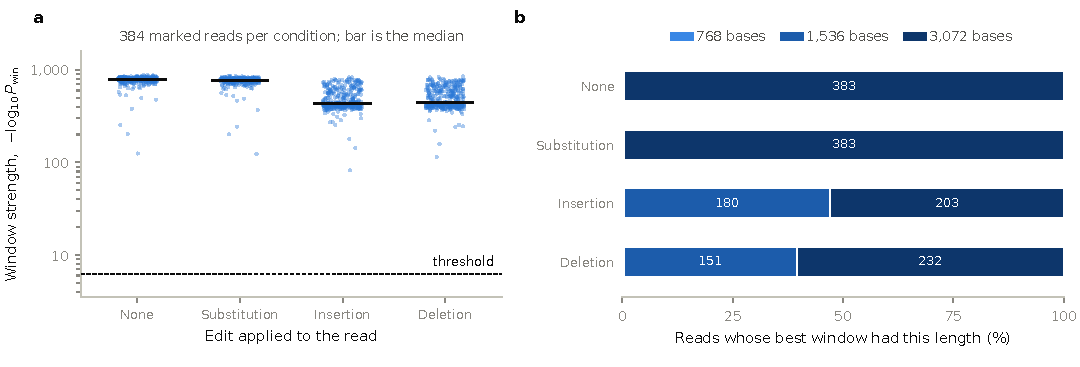
\includegraphics[width=\textwidth]{fig4_edits}
\caption{\textbf{Effects of single-base edits on detection in Carbon.} All panels are Carbon.
\textbf{a}, Strength of the best window in each of the 384 marked reads per condition, on a log
scale, with the median shown as a bar. The dashed line is the detection threshold. Substitution
produces a small reduction in median strength; insertion and deletion reduce it by approximately
half, while all marked reads remain above the threshold.
\textbf{b}, Length of the window that carried the strongest evidence. Numbers inside the bars are
read counts out of 384. The full 3{,}072-base window is strongest for nearly all unedited and
substituted reads. Shorter windows are more frequently selected after insertion or deletion.}
\label{fig:edits}
\end{figure*}

\section{Discussion}

This study integrated the SynthID tournament watermark into Carbon-500M and GENERator-v2 1.2B and
evaluated sampler fidelity, sequence-quality proxies, and position-independent detection. Both
models showed agreement with the intended sampling distribution at the evaluated states, no
statistically detectable differences in the declared quality proxies, and detection of all
held-out marked reads under unedited and tested single-base edit conditions. These findings support
the feasibility of generation-time watermarking and subsequent detection without access to the
model or generation boundary within the evaluated corpus.

A central methodological result is that detection remained effective after explicit correction
for alignment and location uncertainty. The verifier searches both strands, every starting base,
and four window lengths, and includes every tested window in the read-level correction. Carbon's
window-level results show that the signal accumulated over the evaluated continuations substantially
exceeded the corrected threshold. This margin should not be assumed for shorter continuations or
longer surrounding reads: shorter generated regions provide fewer mark bits, while longer reads
increase the number of candidate windows. The minimum detectable continuation length under these
conditions remains to be established.

Applying the same sampler and verifier to two models supports portability across the evaluated
model implementations. The detector depends on the observed read and public settings, so its
statistical procedure is unchanged between Carbon and GENERator. Their agreement in detection
outcomes and the absence of measurable quality loss provide evidence beyond a single model
application. However, the models share the same prompt cohort and token length, limiting
extrapolation to other corpora and tokenisation schemes. This comparison also does not establish
relative biological quality or equivalence between the models.

The Carbon results clarify the role of alignment search after insertions and deletions. A
substitution preserves downstream token boundaries, whereas an insertion or deletion changes the
alignment of every subsequent token within a window spanning the edit. The increased frequency of
shorter strongest windows after these edits is consistent with the verifier selecting regions
whose alignment remains usable. Exhaustive search over starting bases also permits recovery of
the original alignment downstream of an edit. This mechanism supports the observed single-edit
results, but provides no general guarantee against more extensive modification. Theoretical work
on watermark removal further emphasises that robustness depends on the permitted adversarial
capabilities \cite{zhang2024sand}. Here, each read received exactly one randomly specified edit,
without access to the verifier's score.

The alignment problem is related to synchronisation errors in coding theory. Synchronisation
strings explicitly encode indexing information to support recovery from insertions and deletions
\cite{haeupler2017synchronization}. Pseudorandom codes combine computational indistinguishability
with decodability under specified error models, motivating their use in watermarking
\cite{christ2024prc}. Our verifier addresses alignment uncertainty through exhaustive search,
without adding an explicit indexing code to the sequence. The resulting cost is the number of
windows evaluated and the associated multiple-testing correction. This analogy concerns the
alignment problem; it does not imply the error-correction guarantees of those coding constructions.

Watermarking designed coding sequences through synonymous substitution, including approaches that
preserve the mark in translated proteins \cite{zhang2025securing}, addresses a complementary
objective. Such methods assume a coding region and permit explicit sequence modification, whereas
our evaluation concerns detection in generated DNA without those assumptions. Combining these
approaches may support broader provenance workflows, but their compatibility and biological
consequences would require separate evaluation.

\section{Limitations}

The study evaluates two models, one watermark construction, one verifier, and one shared prompt
cohort. Each model contributes a single execution, and independent confirmatory replication remains
outstanding. Both models use six-base tokens, as do other genomic models \cite{wu2025generator};
models with single-base or variable-length tokenisation would present different alignment
requirements. Longer reads would also increase the search correction. Because both models use the
same prompts, the study evaluates portability across models without independent replication across
corpora.

The retained analyses differ in coverage. Carbon provides window-strength distributions,
standardized effects for all 14 sequence measures, and the length of the strongest window after
each edit. GENERator provides the aligned-detector null diagnostic. Claims based on these analyses
are attributed to the corresponding model; the empirical panels in the four figures use Carbon
results.

Generation was performed on GPU hardware and detection on x86-64 CPUs. These results have not been
independently replicated across computing platforms. For the Carbon detection run, the retained
protocol document differs from the protocol hash recorded in the result. This documented
provenance discrepancy remains unresolved and limits verification of the executed protocol.
Confirmatory replication is required to address these execution and provenance limitations.

The observed false-positive counts are compatible with the 1\% target but do not establish an
operational rate below it. Among 192 independent prompts, Carbon had one ordinary positive and no
wrong-key positives; GENERator had one wrong-key positive and no ordinary positives in the
unedited condition. The confidence interval for one positive prompt extends to 2.87\%, and the
upper bound for zero positives is 1.90\%. More independent prompts are needed to estimate rates
near the declared target precisely.

The experiments use published keys for reproducibility and therefore do not evaluate secrecy or
resistance to key recovery in deployment. The analytic null also relies on the modelling assumption
that mark bits behave as independent fair binary values without the correct key. Adaptive prompting
has recovered keyed sequences in text watermarking \cite{reynolds2025breaking}, and model queries
have enabled watermark forgery and removal \cite{jovanovic2024stealing}. Whether these attacks
transfer to the evaluated genomic setting is untested. The assumed attacker does not hold the key
and cannot observe or query the verifier's score.

Finally, model likelihood and sequence statistics are biological proxies. They do not measure
expression, replication, function, viability, or safety. The absence of detectable changes in these
measures therefore does not establish preservation of biological function. Addressing that
limitation requires experimental assays.

\section{Conclusion}

The SynthID tournament watermark was applied to Carbon-500M and GENERator-v2 1.2B without a
statistically detectable loss in the evaluated model-likelihood and sequence-quality proxies.
Position-independent verification detected all 384 held-out marked reads per model in the
unedited condition and after each tested single-base substitution, insertion, or deletion, with
read-level correction over both strands, every starting base, and four window lengths. Control
counts were compatible with the declared false-positive target, although 192 independent prompts
provide limited precision near a 1\% rate. Carbon's window-level analyses further support
alignment recovery through the search after insertions and deletions. These findings support the
feasibility of statistical provenance detection in model-generated DNA within the evaluated scope,
with independent replication, broader sequence coverage, and biological validation remaining
necessary next steps.

\section*{Data and code availability}

The two experimental keys are published as public fixtures for reproducibility. They are not
deployment secrets, and the experiments do not assess resistance to secret-key recovery. The
generated sequences, verifier outputs underlying the figures, prompt set, and analysis and figure
code are available from the authors on request.

\bibliographystyle{plain}
\bibliography{refs}

\end{document}
